% --- Appendix ---
\chapter{The first appendix}
% ---feference ---
\section{รายการอ้างอิง (References)}

\textbf{Andrew Lucas.} (2014). \textit{Ising formulations of many NP problems.} วิทยานิพนธ์, Department of Physics, Harvard University, Cambridge, MA, USA 02138.

\textbf{Dax Enshan Koh, Kaavya Kumar, และ Siong Thye Goh.} (2024). \textit{Quantum Volunteer’s Dilemma.} วิทยานิพนธ์, Singapore Management University.

\textbf{Jedsadakorn Kritsadakul และ Sanpawat Kantabutra.} (2025). \textit{Hybrid classical quantum computation for cybersecurity strategies in a layered cybersecurity model.} วิทยานิพนธ์, Chiang Mai University.

\textbf{Kaushik Naskar.} (2021). \textit{Quantum version of Prisoners' Dilemma under Interacting Environment.} วิทยานิพนธ์, Department of Physics, Taki Government College.

\textbf{Kay-Yut Chen และ Tad Hogg.} (2006). \textit{How Well Do People Play a Quantum Prisoner’s Dilemma?} Quantum Information Processing, 5(1), กุมภาพันธ์ 2006.

\textbf{Vitis Technologies.} (n.d.). \textit{What is Layered Security \& How Does it Defend Your Network?} สืบค้นเมื่อ 1 กันยายน 2025 จาก  
\url{https://www.vitistech.com/posts/what-is-layered-security-how-does-it-defend-your-network}




% --- คู่มือการใช้งานระบบ ---
\chapter{\ifenglish System Manual\else คู่มือการใช้งานระบบ\fi}

ในบทนี้จะอธิบายถึงรายละเอียดการติดตั้งและการใช้งานระบบวิเคราะห์ดุลยภาพแนช (Nash Equilibrium Analysis System) โดยใช้เทคนิคการคำนวณแบบไฮบริดระหว่างคอมพิวเตอร์แบบดั้งเดิมและคอมพิวเตอร์ควอนตัมจำลอง เพื่อให้ผู้ใช้สามารถนำไปประยุกต์ใช้ในการวิเคราะห์กลยุทธ์ด้านความมั่นคงปลอดภัยไซเบอร์ได้อย่างถูกต้อง

% ---บอกว่าควรใช้ Google Colab ---
\section{สภาพแวดล้อมสำหรับการประมวลผล (Execution Environment)}
ผู้วิจัยเสนอแนะให้ดำเนินงานผ่านทาง \textbf{Google Colab} ซึ่งเป็นแพลตฟอร์มบนระบบคลาวด์ที่มีประสิทธิภาพสูงสำหรับการประมวลผลอัลกอริทึมเชิงคำนวณ โดยมีข้อดีและขั้นตอนการใช้งานดังนี้
\begin{itemize}
    \item \textbf{การเตรียมการ:} ผู้ใช้สามารถเริ่มต้นใช้งานได้ทันทีโดยไม่ต้องตั้งค่าสภาพแวดล้อม (Environment) ภายในเครื่องคอมพิวเตอร์ส่วนบุคคล 
    \item \textbf{การเชื่อมต่อทรัพยากร:} รองรับการเชื่อมต่อกับ Google Drive เพื่อจัดเก็บโค้ดโปรแกรมและตารางผลตอบแทน (Payoff Tables) ได้อย่างเป็นระบบ 
    \item \textbf{ความพร้อมของไลบรารี:} รองรับการติดตั้งไลบรารีสำหรับการคำนวณควอนตัมจำลอง เช่น \texttt{dimod} และ \texttt{pyqubo} ได้โดยตรงผ่านระบบจัดการแพ็กเกจ 
\end{itemize}



% --- การติดตั้งไลบรารี ---
\section{ขั้นตอนการใช้งานระบบ (Operating Procedures)}
\begin{enumerate}
    \item \textbf{การติดตั้งไลบรารีหลัก:} ดำเนินการติดตั้งผ่านคำสั่ง pip ใน Terminal หรือ Code Cell
    % ---โค้ด ---
    \begin{lstlisting}[language=Python]
    !pip install dimod pyqubo dwave-neal
    \end{lstlisting}
    % ---แปะรูปโค้ดการติดตั้งไลบรารี ---
    \begin{center}
    
\includegraphics{pipCodeCell.png}
    \end{center}


    \item \textbf{หน้าที่ของไลบรารี:}
    \begin{itemize}
        \item \textbf{dimod:} สำหรับการจัดการโครงสร้างปัญหาในรูปแบบ Binary Quadratic Model (BQM)
        \item \textbf{pyqubo:} สำหรับการสร้างตัวแปร Binary และการแปลงสมการทางคณิตศาสตร์ให้อยู่ในรูปแบบ QUBO
        \item \textbf{neal:} สำหรับการประมวลผลผ่านอัลกอริทึม Simulated Annealing Sampler
    \end{itemize}

    % ---แปะรูปโค้ดไลบรารี ---
    \begin{center}
    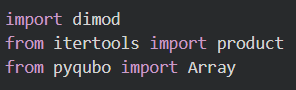
\includegraphics{libraryCode.png}
    \end{center}
\end{enumerate}

% --- ข.3 ---
\section{การกำหนดค่าเริ่มต้นและข้อมูลนำเข้า (Data Configuration)}
ผู้ใช้สามารถกำหนดตารางผลตอบแทน (Payoff Table) โดยแบ่งตามรูปแบบของผู้เล่นในระบบ ดังนี้

\subsection{การกำหนดค่าสำหรับผู้เล่น 3 คน (3-Player Game)}
โครงสร้างข้อมูลจะต้องถูกจัดเก็บในรูปแบบ Dictionary โดยระบุกดุลยภาพพื้นฐานของฝ่ายป้องกัน (Defender Strategies) เป็นคีย์หลัก
\begin{lstlisting}[language=Python]
tables = {
    "ASC": [[(A1, A2, D), (A1, A2, D)], [(A1, A2, D), (A1, A2, D)]],
    "DSC": [[(A1, A2, D), (A1, A2, D)], [(A1, A2, D), (A1, A2, D)]],
    "Random": [[(A1, A2, D), (A1, A2, D)], [(A1, A2, D), (A1, A2, D)]]
}
\end{lstlisting}
โดยที่ค่าใน Tuple หมายถึงผลตอบแทนของผู้โจมตีรายที่ 1, ผู้โจมตีรายที่ 2 และผู้ป้องกัน ตามลำดับ
    % ---แปะรูปโค้ดตาราง table ---
\begin{figure}[H]
    \centering
    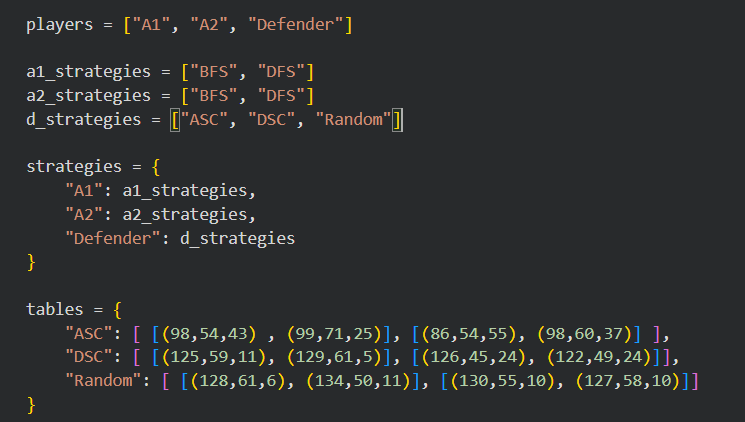
\includegraphics[width=0.8\textwidth]{TableCode.png}
    \caption{การกำหนดตารางผลตอบแทนและกลยุทธ์ในรูปแบบ Python Dictionary}
    % \label{fig:table_code}
\end{figure}

% --- ข.4 ---
\section{กระบวนการประมวลผลหลัก (Core Processing)}
การทำงานของระบบจะแบ่งออกเป็นขั้นตอนสำคัญที่ผู้ใช้สามารถปรับแต่งค่าพารามิเตอร์ได้ ดังนี้

\begin{enumerate}
    \item \textbf{การกำหนดขนาด Slack Variable:} ปรับค่า \texttt{num\_bits} เพื่อรองรับช่วงความต่างของผลตอบแทน (เช่น 5 บิต สำหรับส่วนต่างไม่เกิน 31 หรือ 7 บิต สำหรับส่วนต่างไม่เกิน 127)

    % -- -แปะรูปโค้ด Slack Variable ---
    \begin{figure}[H]
    \centering
    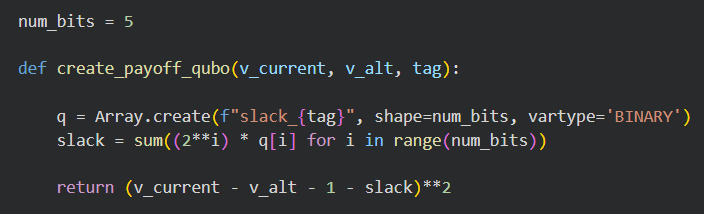
\includegraphics[width=\textwidth]{ SlackCode.png}
    \caption{การกำหนดขนาด Slack Variable}
    % \label{fig:table_code}
    \end{figure}

    \item \textbf{การสร้างสมการ QUBO:} ระบบจะใช้ฟังก์ชัน \texttt{create\_payoff\_qubo} เพื่อแปลงความสัมพันธ์ระหว่างผลตอบแทนปัจจุบันและผลตอบแทนทางเลือกให้อยู่ในรูปสมการกำลังสอง $(V_{current} - V_{alt} - 1 - Slack)^2$
    
    % QUBOcode.png
    % -- -แปะรูปโค้ด Slack Variable ---
    \begin{figure}[H]
    \centering
    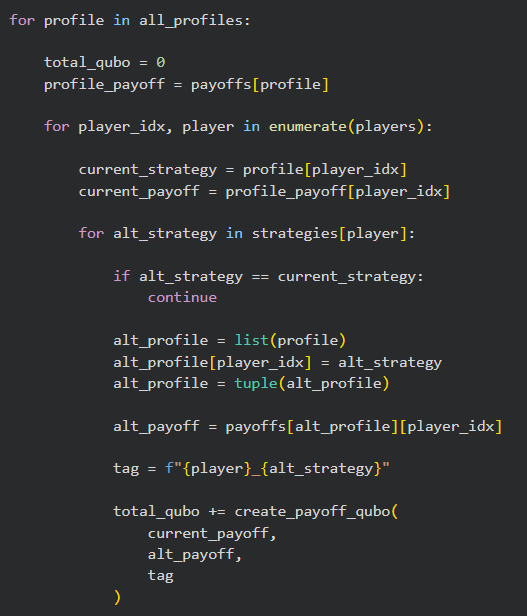
\includegraphics[width=0.8\textwidth]{QUBOcode.png}
    \caption{การสร้างสมการ QUBO จากตารางผลตอบแทนและการกำหนด Slack Variable}
    % \label{fig:table_code}
    \end{figure}

    \item \textbf{การเลือก Solver:} 
    \begin{itemize}
        \item สำหรับปัญหาขนาดเล็ก: แนะนำให้ใช้ \texttt{dimod.ExactSolver()} เพื่อหาคำตอบที่แม่นยำที่สุด
        \item สำหรับปัญหาขนาดใหญ่: แนะนำให้ใช้ \texttt{neal.SimulatedAnnealingSampler()} เพื่อเพิ่มประสิทธิภาพในเชิงเวลา
    \end{itemize}
    % SolverCode.png
    % -- -แปะรูปโค้ด Solver ---
    \begin{figure}[H]
    \centering
    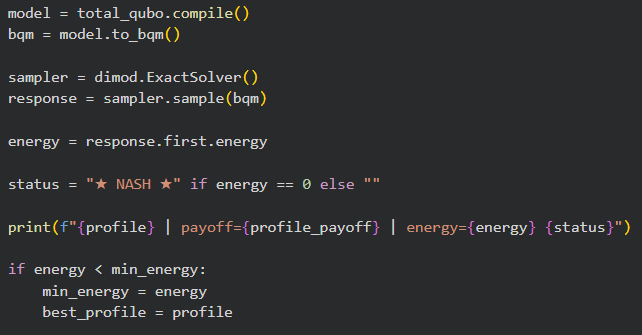
\includegraphics[width=0.8\textwidth]{SolverCode.png}
    \caption{การเลือก Solver สำหรับการประมวลผล QUBO}
    % \label{fig:table_code}
    \end{figure}
\end{enumerate}



% --- ข.5 ---
\section{การตีความผลลัพธ์ (Output Interpretation)}
เมื่อระบบดำเนินการประมวลผลเสร็จสิ้น ผลลัพธ์จะถูกแสดงผลในรูปแบบตารางเปรียบเทียบค่าพลังงาน (Energy) ดังนี้

\begin{itemize}
\item \textbf{สถานะ {\fontspec{TeX Gyre Termes}★} NASH {\fontspec{TeX Gyre Termes}★}:} ปรากฏเมื่อค่าพลังงานของโปรไฟล์กลยุทธ์นั้นเท่ากับ $0.0$ ซึ่งหมายความว่าเป็นจุดดุลยภาพที่เหมาะสมที่สุด
    \item \textbf{ค่าพลังงาน (Energy):} หากค่าพลังงานมีค่ามากกว่า $0$ แสดงว่าโปรไฟล์นั้นไม่ใช่ดุลยภาพแนช โดยค่าพลังงานที่แสดงจะสะท้อนถึงระดับความเสียดาย (Regret) ของผู้เล่นในระบบ
    \item \textbf{สรุปผล (Summary):} ระบบจะแสดงจุดดุลยภาพแนชที่ดีที่สุดพร้อมค่าผลตอบแทนรวมในส่วนท้ายของการประมวลผล
\end{itemize}

% resultEx.png
% ภาพตัวอย่างผลลัพธ์ 
    \begin{figure}[H]
    \centering
    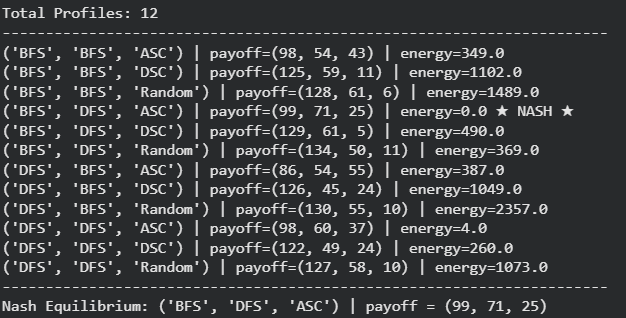
\includegraphics[width=0.8\textwidth]{resultEx.png}
    \caption{ภาพตัวอย่างผลลัพธ์การประมวลผลที่แสดงสถานะ NASH และค่าพลังงานของโปรไฟล์กลยุทธ์ต่าง ๆ}
    % \label{fig:table_code}
    \end{figure}